\documentclass{article} % Oder eine andere Dokumentklasse wie report, book, etc.
\usepackage[utf8]{inputenc} % Bestimmt die Eingabe-Kodierung
\usepackage[T1]{fontenc} % Bestimmt die Ausgabe-Kodierung
\usepackage{graphicx}


\begin{document}
	
	\title{Deep Reinforcement Learning Exercise 02}
	\maketitle
	
	Group:
	\begin{itemize}
		\item Marvin Kohnen
		\item Moritz Gehring
		\item Julius Ferber 
		
	\end{itemize}
	\section{Exercise 3.1}

	\subsection{3.1a}
		Figure \ref{fig:1} shows the State Value functions and final optimal policy for the implemented GPI algorithm. Note that we reach state values of up to 45 in the best states (yellow). 
	\begin{figure}[h!]
		\centering
		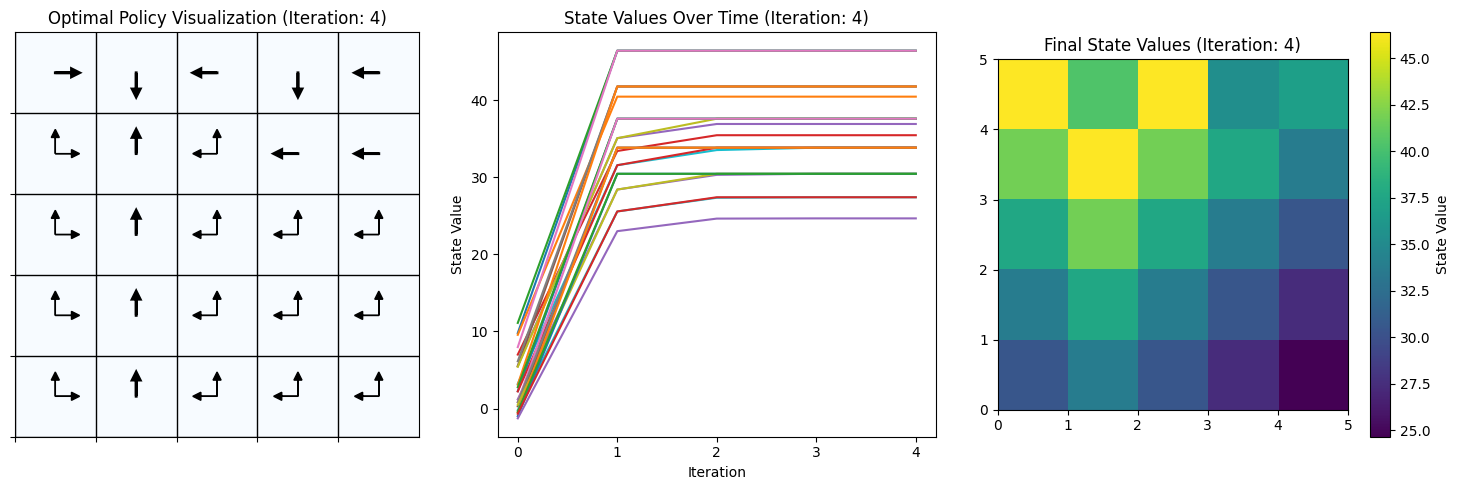
\includegraphics[width=0.9\textwidth]{images/3.1a.png}
		\caption{State Value functions and final optimal policy visualization}
		\label{fig:1}
	\end{figure}
	
	\subsection{3.1b}
	 
 	While using general policy iteration, the policy converges very stably and quickly in only a couple of iterations (see Figure \ref{fig:1}). On the other hand, when using value iteration, the policy converges gradually and therefore much more slowly, but also equally reliably (see middle image of Figures \ref{fig:2} to \ref{fig:5}). 
	Of course, value iteration is much more computationally inexpensive than policy iteration, since it only evalueates the value function once each iteration.  As we can see though, the values reached in the final iteration are not as good as the ones reached using general policy iteration. Compared to the aforementioned state values for GPI (45 for the yellow states), the value iteration algorithm only reaches state values aorund 23. This is the case because the policy is updated right after on evaluation step, and not after the value function has converged.
	
	In the end, both methods get to the same optimal policy (compare left most picture in Figures \ref{fig:1} and \ref{fig:5}).
	
	\begin{figure}[h!]
		\centering
		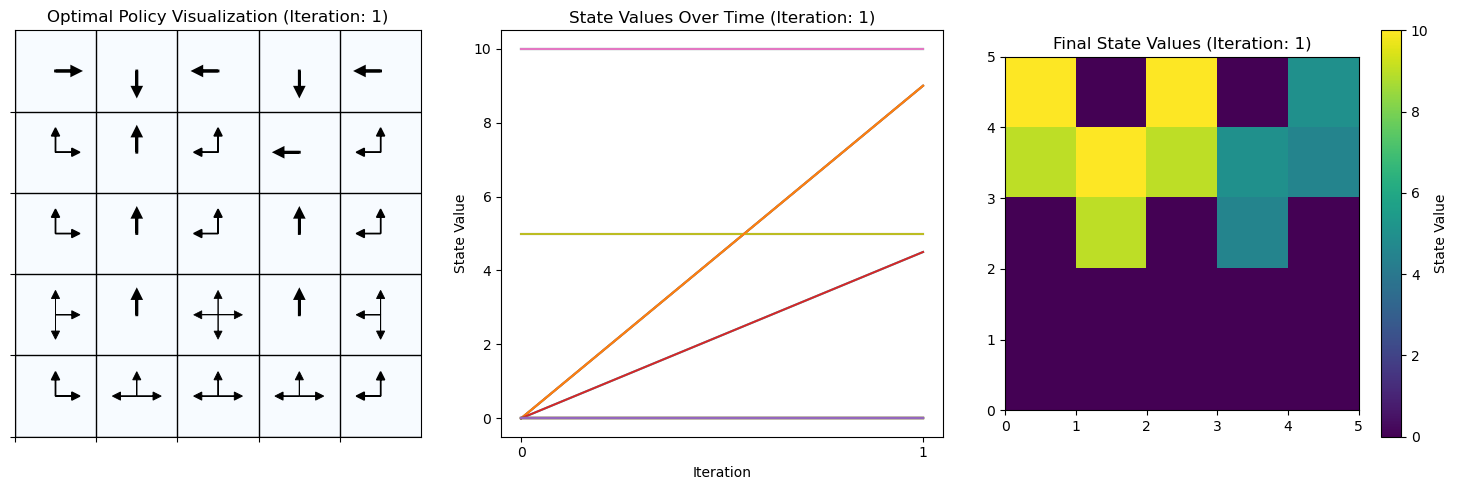
\includegraphics[width=0.9\textwidth]{images/3.1b.1.png}
		\caption{State Value functions and final optimal policy visualization after iteration 1}
		\label{fig:2}
	\end{figure}
	
		\begin{figure}[h!]
		\centering
		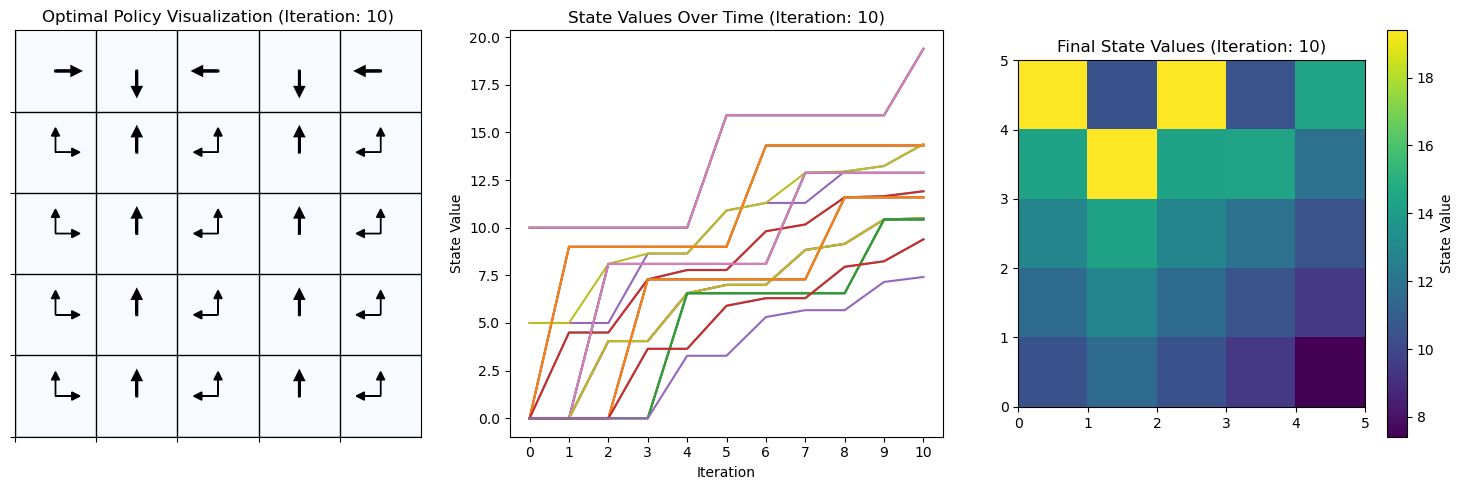
\includegraphics[width=0.9\textwidth]{images/3.1b.2.png}
		\caption{State Value functions and final optimal policy visualization after iteration 10}
		\label{fig:3}
	\end{figure}
	
	
	\begin{figure}[h!]
		\centering
		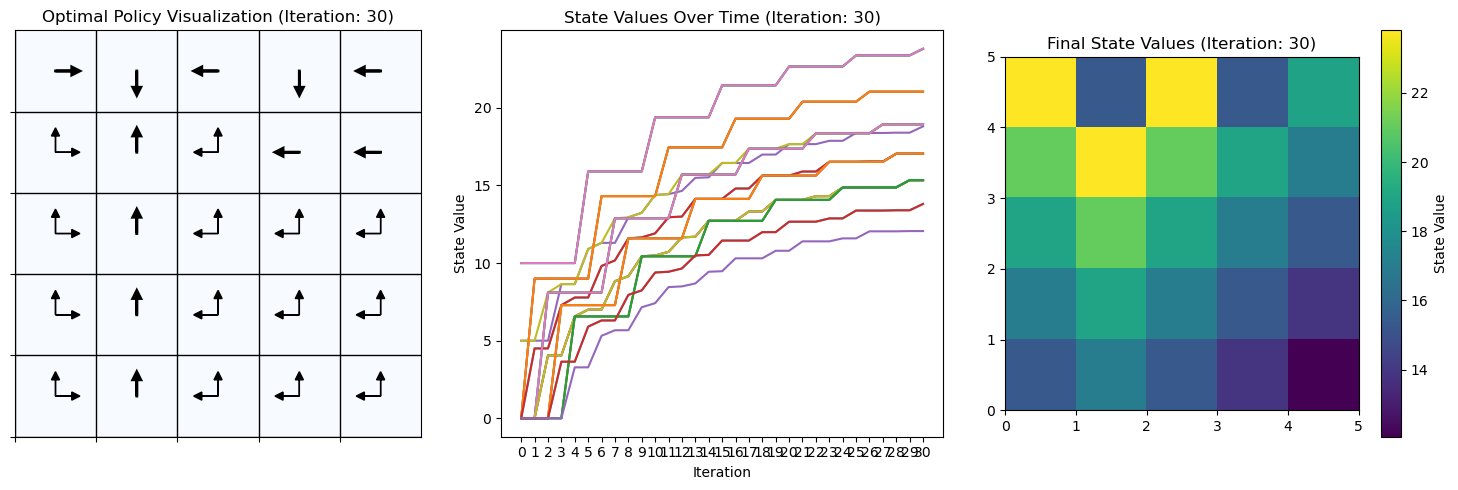
\includegraphics[width=0.9\textwidth]{images/3.1b.3.png}
		\caption{State Value functions and final optimal policy visualization after iteration 30}
		\label{fig:4}
	\end{figure}
	
	\begin{figure}[h!]
		\centering
		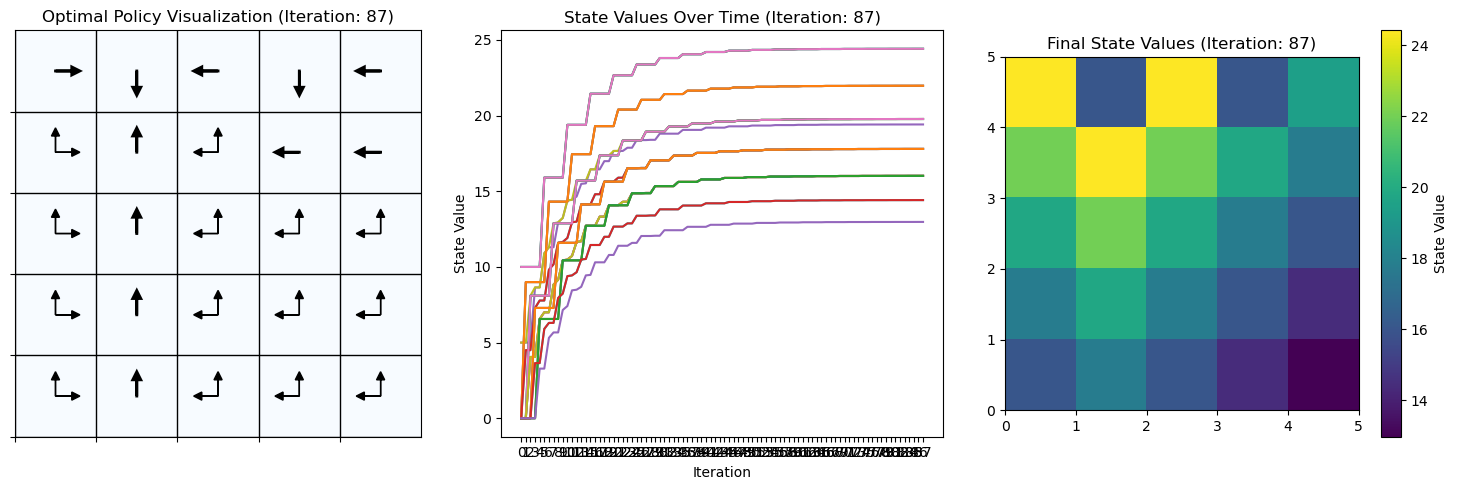
\includegraphics[width=0.9\textwidth]{images/3.1b.4.png}
		\caption{State Value functions and final optimal policy visualization after iteration 87}
		\label{fig:5}
	\end{figure}
	
	\newpage
	
	\subsection{3.1c}
	\textbf{Conceptual difference for GPI with Value function}: \newline
	When using the action value function, we are taking the max over all actions for each state, and then updating the value function for each state. Regarding the State-value function, we're updating the value function for each state based on the expected return of each action in that state.\newline
	\textit{Moving on to the analysis}: \newline
	Interestingly, the policy doesnt converge to the same optimal policy as in the previous exercises, but to a slightly different one. It looks like the policy using the action values has a smaller "scope", since the decision to go into the B cycle is made using action value functions for the whole column 3, while using state value functions, the A cycle is preferred for position (1, 3). 
	The convergence seems to be of similar speed to the one using state value functions, since the number of policy iterations is again only 3, while the number of iterations to evaluate the action values is 89 (see \ref{fig:11}), like when using state value functions.
	
	
	\begin{figure}[h!]
		\centering
		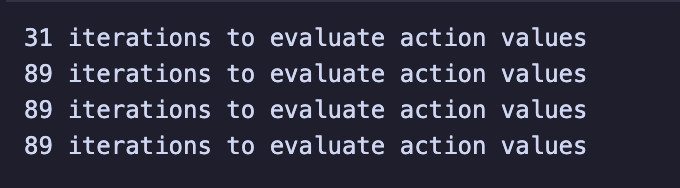
\includegraphics[width=0.9\textwidth]{images/3.1c.4.png}
		\caption{Logging output monitoring iterations to evaluate action values.}
		\label{fig:11}
	\end{figure}
	
	\begin{figure}[h!]
		\centering
		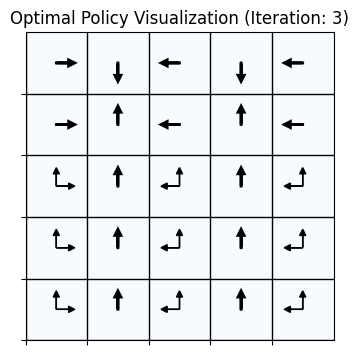
\includegraphics[width=0.9\textwidth]{images/3.1c.1.png}
		\caption{Optimal policy visualization}
		\label{fig:6}
	\end{figure}
	
	\begin{figure}[h!]
		\centering
		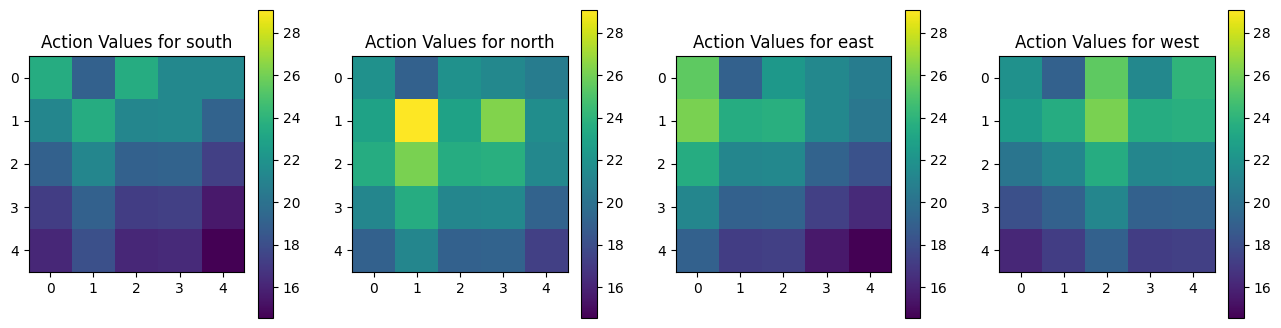
\includegraphics[width=0.9\textwidth]{images/3.1c.2.png}
		\caption{Action values by direction}
		\label{fig:7}
	\end{figure}
	\begin{figure}[h!]
		\centering
		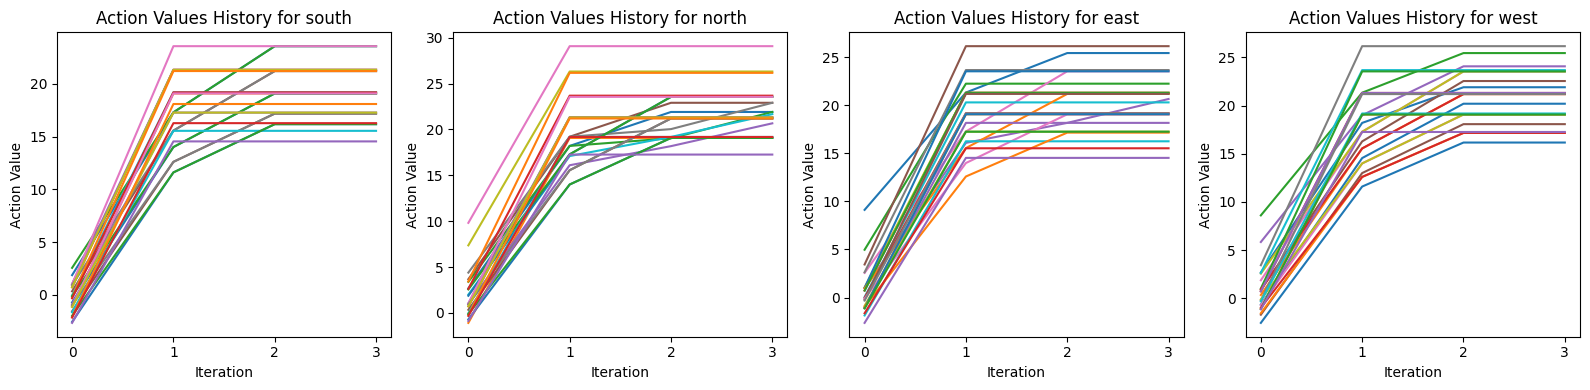
\includegraphics[width=0.9\textwidth]{images/3.1c.3.png}
		\caption{Optimal policy visualization}
		\label{fig:8}
	\end{figure}
	\clearpage
	\section{Exercise 3.2}

	\subsection{3.2.a}
	
	The initial policy is defined with the following probabilities:
	\begin{itemize}
		\item Moving RIGHT: 35\%
		\item Moving DOWN: 35\%
		\item Moving LEFT: 15\%
		\item Moving UP: 15\%
	\end{itemize}
	
	The rationale behind this policy is that, as the goal is located at the bottom right of the lake and the starting point is at the top left, the general strategy should be to move towards the bottom-right direction.
	
	When applying Monte Carlo prediction in the context of Reinforcement Learning, the characteristics that an initial policy must have are:
	
	1. \textbf{Coverage of entire State-Action Space}: The policy should be able to visit all relevant states and state-action pairs. Ensuring that all areas of the state-action space are covered ensures that the estimated values are accurate.
	
	2. \textbf{Consistency with Problem Constraints}: The initial policy should respect any constraints inherent in the problem domain (eg. using only valid movement commands in this case). 
	
	3. \textbf{Exploratory nature} The initial policy should ensure sufficient exploration of the state space.
	
	Our policy  adequately reflects all 3 characteristics. 
	\newline
	
	
	
	\textit{Moving on to the Analysis part}:
		
	A state value is only the average action value in that state across all actions and the policy
	However, if the state has an action that guarantees a reward (e.g. the action to the left of the goal, 
	in this case with a value of ~0.6 - see Figure \ref{fig:9}), that fact is not accurately represented by just the state value function
	Similarly, states far from the goal are all evaluated very close to each other in value (in this case 0),
	even though some of them are clearly superior (e.g. tile 6 compared to tile 4), but since the agent generally
	fails to retrieve a reward very often, they have almost the same value.
	
	\begin{figure}[h!]
		\centering
		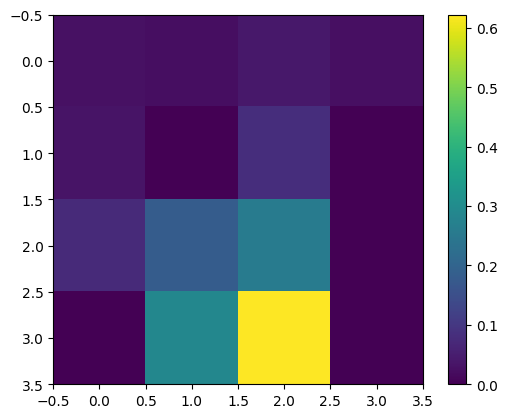
\includegraphics[width=0.9\textwidth]{images/3.2a.png}
		\caption{Monte Carlo Heatmap}
		\label{fig:9}
	\end{figure}
	
	\subsection{3.2.b}
	
	The visualization of the On-Policy Monte Carlo can be seen in Figure \ref{fig:10} and the optimal policy in Figure \ref{fig:12}. We also plotted the heatmap for each action in Figure \ref{fig:13}
	
	Even though in (3,2), the action RIGHT should give a reward of 1 every time, because it is slippery and there is a randomness factor, its state-action value is less than 1 (Figure \ref{fig:13}).
	Controversely, the action value for the action DOWN is actually sometimes greater than the one for RIGHT. This is because the discounting factor `gamma` is 1 (i.e. there is no discounting), and because when using the action DOWN in (3,2), there is a chance that the agent slips into the goal state, and if not, it either slips into another safe state (there are no adjacent holes) or stays in (3,2).
	Therefore, the calculated action values can only be relied upon to a certain extent, as the best action in (3,2) is obviously to move RIGHT, but due to the non-deterministic environment dynamics, this will not always be represented in the state-action values.
	
	\begin{figure}[h!]
		\centering
		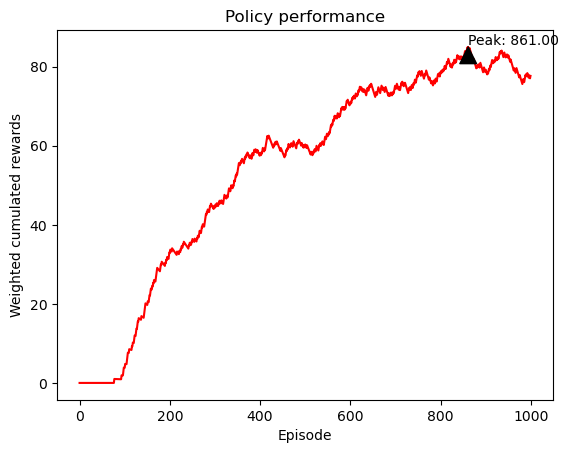
\includegraphics[width=0.9\textwidth]{images/3.2b.1.png}
		\caption{Monte Carlo Policy Performance}
		\label{fig:10}
	\end{figure}
	
	
	\begin{figure}[h!]
		\centering
		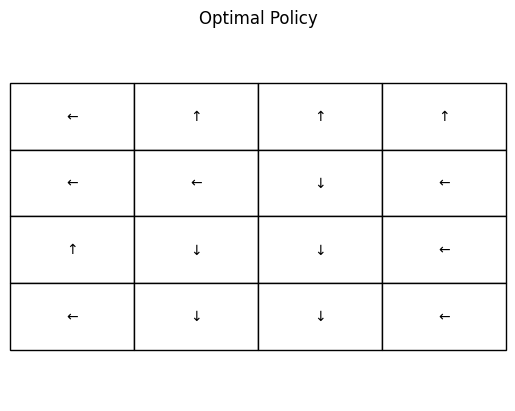
\includegraphics[width=0.9\textwidth]{images/3.2b.2.png}
		\caption{Optimal Policy for On-policy Monte Carlo Control}
		\label{fig:12}
	\end{figure}
	
		\begin{figure}[h!]
		\centering
		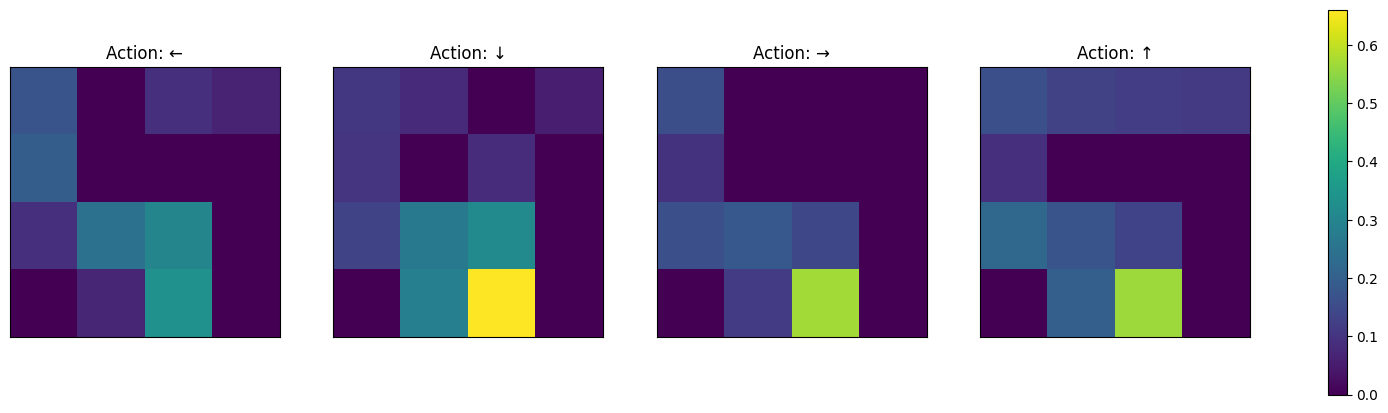
\includegraphics[width=0.9\textwidth]{images/3.2b.3.png}
		\caption{Heatmap for each Action}
		\label{fig:13}
	\end{figure}
	
	\subsection{3.3}
	I'm so sorry boys, but i'm \textbf{fucking cooked}. 
	
	
\end{document}